\section{Introduction}

Multivariate long-term time series forecasting predicts future dynamics from multichannel historical observations and supports applications such as energy scheduling, weather monitoring, traffic management, and industrial operations \citep{Lim2021DeepForecastSurvey}. Models must capture the temporal evolution of individual variables and cross-variable dependencies while maintaining predictive accuracy over extended horizons. Recent approaches have explored sparse attention, series decomposition, patch-based representations, variable tokens, and multiscale modeling \citep{Wen2023TransformerSurvey,Zhou2021Informer,Wu2021Autoformer,Nie2023PatchTST,Liu2024iTransformer,Wu2023TimesNet,Wang2024TimeMixer}. Nevertheless, as available observations extend further into the past, extracting stable and informative signals from increasingly long histories remains a central challenge.

Extending the lookback window can expose long-period patterns and slow state changes, but it can also introduce redundancy, noise, state mismatch, and additional computational cost. The Maximum Effective Window (MEW) study showed that, for the evaluated Transformer-based forecasters, increasing the input window beyond a certain range did not necessarily improve performance; it therefore employed information filtering and selective forgetting to improve the use of long histories \citep{Zhang2025MEW}. This observation suggests that long-context forecasting should account not only for the number of available observations but also for the roles of observations at different temporal positions. Observations near the forecast origin often characterize the current predictive state more directly, whereas earlier observations may be better suited to providing periodic context, historical states, and information about potential biases. If all temporal ranges are processed at the same resolution by a single computationally intensive backbone, the use of historical information and the associated computational cost cannot be adjusted independently.

Existing approaches exploit the heterogeneity of historical information from several perspectives. NHITS, Pathformer, MICN, MCNet, and AweHF organize different frequencies, temporal resolutions, signal components, or receptive fields through hierarchical interpolation, multiscale branches, signal decomposition, and local--global modeling \citep{Challu2023NHITS,Chen2024Pathformer,Wang2023MICN,Sun2024MCNet,Gong2026AweHF}. Attraos, PFRP, and RAFT augment the current input using dynamical-system memories or external historical retrieval \citep{Hu2024Attraos,Du2026PFRP,Han2025RAFT}. DualNet, Multi-Granularity Residual Learning, xLSTM-Mixer, and PIR improve a base forecast through compensation, residual refinement, or instance-level revision \citep{Li2025DualNet,Hou2022MRLF,Kraus2025xLSTMMixer,Liu2025PIR}. These studies primarily concern the representation scale, retrieval strategy, and fusion mechanism of historical information. The temporal distance between a historical observation and the forecast origin, however, has not been explicitly used to assign distinct predictive roles.

Motivated by this gap, we propose TimeRole, a history-role-differentiated model for multivariate long-term forecasting. TimeRole partitions the input into a recent window and distant history. The recent window retains its original resolution and is processed by a recent graph-enhanced state-space predictor (RGSP), which estimates the current predictive state and produces a complete base forecast. The distant-history corrector (DHC) compresses earlier observations at a lower resolution and, conditioned on the same recent state, forms a conditional correction from the difference between paired outputs of a shared decoder. A bounded variable-wise coefficient then injects this correction into the base forecast. This asymmetric architecture allows the accessible historical range and the sequence length directly processed by the computationally intensive forecasting backbone to be controlled separately. RGSP combines graph learning and selective state-space modeling to capture recent temporal dynamics and cross-variable relationships \citep{Huang2023CrossGNN,Wang2025SMamba,Karadag2026msMamba,Chen2026GMamba,Zhou2026SSMGNN}, while DHC supplements the prediction with compressed distant-history information.

Experiments on five public datasets and four prediction horizons demonstrate that TimeRole achieves competitive overall performance. Under the three-seed evaluation, TimeRole produced lower test errors than the recent-only RGSP-96 in all eight tasks on ETTm1 and ETTm2. Performance generally deteriorated when the distant history was mismatched across samples, temporally shuffled, reversed, or replaced, indicating that the conditional correction used distant information associated with the current sample. When integrated into TimeXer, DHC also yielded lower errors than the direct long-input configuration on most tasks while retaining parameter counts and GPU memory consumption close to those of the short-input backbone. Collectively, these results support history-role differentiation as a means of exploiting longer histories while controlling computational cost.

Our main contributions are as follows:

\begin{enumerate}
\def\labelenumi{\arabic{enumi}.}
\tightlist
\item
  We introduce TimeRole and a strategy that differentiates the predictive roles of recent and distant history. By separating high-resolution base forecasting from low-resolution historical correction, TimeRole expands the accessible historical range without increasing the sequence length directly processed by RGSP.
\item
  We develop DHC as a functional complement to RGSP. Distant-history compression, shared-decoder differencing under the same recent state, and bounded variable-wise injection form a conditional correction pathway designed to express distant history as an incremental adjustment to the base forecast.
\item
  We evaluate TimeRole through unified baseline comparisons, multi-seed controls, distant-history interventions, cross-backbone transfer, and resource measurements. The results show that the model can use distant history matched to the current sample and achieve a favorable balance between predictive accuracy and computational cost.
\end{enumerate}

\section{Related Work}

\subsection{Long-term forecasting backbones and heterogeneous temporal structures}

Long-term forecasting models have primarily addressed the representation of long-range dependencies, computational efficiency, and direct multi-step prediction \citep{Lim2021DeepForecastSurvey,Wen2023TransformerSurvey}. In addition to complex deep architectures, DLinear provides a competitive simple baseline using linear mappings after trend--seasonal decomposition, whereas NHITS progressively combines forecast components at different frequencies through multi-rate sampling and hierarchical interpolation \citep{Zeng2023DLinear,Challu2023NHITS}. These studies indicate that input organization and forecast decomposition, as well as model capacity, affect long-term forecasting performance.

Transformer-based approaches improve long-term forecasting mainly through attention efficiency, sequence organization, and variable interaction. Informer uses ProbSparse attention to reduce the attention cost for long sequences, while Autoformer and FEDformer combine trend--seasonal decomposition with autocorrelation or frequency-domain enhancement, respectively \citep{Zhou2021Informer,Wu2021Autoformer,Zhou2022FEDformer}. PatchTST encodes local patches as tokens, iTransformer represents entire variable series as tokens, and Crossformer explicitly models cross-time and cross-variable dependencies using hierarchical attention \citep{Nie2023PatchTST,Liu2024iTransformer,Zhang2023Crossformer}. These methods improve how historical sequences are represented before entering a unified forecasting backbone, but do not further differentiate the roles of observations at different temporal positions in generating the output.

Multiscale approaches further exploit structures that emerge at different temporal resolutions. TimesNet reshapes one-dimensional sequences into multiple period-aligned two-dimensional representations, and TimeMixer decomposes and mixes information across several sampling scales. Pathformer organizes local and global dependencies through different patch resolutions and adaptive pathways, whereas MICN uses multiscale convolutional branches to extract local features and global correlations \citep{Wu2023TimesNet,Wang2024TimeMixer,Chen2024Pathformer,Wang2023MICN}. MPGTimer jointly models multiscale patches and variable graphs, while MPFGSN uses multi-resolution hyperpatch graphs and frequency-domain graph propagation to organize spatiotemporal relationships \citep{Duan2026MPGTimer,Zheng2025MPFGSN}. These methods organize historical information by scale or pathway, with the resulting representations typically contributing jointly to the complete forecasting objective.

Another line of work constructs separate pathways according to receptive field or signal component. MCNet processes recent segments and variable interactions through a local branch while modeling long-range dependencies over the full sequence through a global branch. Wrinkles in Time uses multiscale two-dimensional patches and a trend super-resolution module to process seasonal and trend components, respectively. AweHF adaptively decomposes low-frequency trends and high-frequency events and models dynamic variable relationships for the event component \citep{Sun2024MCNet,Chen2026Wrinkles,Gong2026AweHF}. TimeRole also adopts differentiated information pathways, but partitions the input according to temporal distance from the forecast origin: the recent window produces a complete forecast, whereas distant history provides a conditional correction.

\subsection{Graph- and state-space-based multivariate forecasters}

Multivariate forecasting also requires the modeling of dependencies among variables. Crossformer connects temporal segments and variables through cross-dimension attention, TPGNN describes dynamic correlations using temporal polynomial graphs, CrossGNN handles heterogeneous interactions through cross-scale and cross-variable graphs, and DiM combines difference-inverted embedding with multi-head graph learning \citep{Zhang2023Crossformer,Liu2022TPGNN,Huang2023CrossGNN,Mo2026DiM}. These methods use attention or graph structures to strengthen the ability of temporal encoders to represent variable relationships.

State-space models provide a near-linear-complexity backbone for long sequences. Mamba regulates information propagation through input-dependent selective state updates, S-Mamba applies bidirectional Mamba to multivariate forecasting, and ms-Mamba represents multiple temporal scales using Mamba blocks with different sampling rates \citep{Gu2024Mamba,Wang2025SMamba,Karadag2026msMamba}. G-Mamba further incorporates static and dynamic graph information into selective state updates, while SSMGNN combines state-space filtering with graph spectral operators \citep{Chen2026GMamba,Zhou2026SSMGNN}. Building on these studies, RGSP combines parameter-shared dual-scale Mamba encoding with variable-graph propagation to model recent temporal dynamics and variable relationships, thereby providing the base forecast for history-role differentiation.

\subsection{Historical memory, retrieval augmentation, and forecast correction}

Methods that directly exploit longer histories mainly focus on historical selection, structured memory, and external retrieval. MEW formalizes the maximum effective window and reduces redundancy and interference in long inputs through information-bottleneck filtering and selective forgetting, whereas Attraos constructs multi-resolution dynamical memory through phase-space reconstruction to support local-evolution forecasting with historical dynamics \citep{Zhang2025MEW,Hu2024Attraos}. PFRP retrieves similar histories from a global memory bank, generates a global forecast, and combines it with a local predictor. RAFT retrieves similar inputs and their subsequent values from the training set as additional historical information for forecasting \citep{Du2026PFRP,Han2025RAFT}. By contrast, TimeRole uses distant history from the same input window. It neither relies on an external historical repository nor produces a separate global forecast alongside the local prediction; instead, it uses distant history to conditionally correct the recent base forecast.

Forecast-correction methods progressively refine predictions through multistage or multi-path architectures. DualNet decouples primary-trajectory estimation from local residual compensation, Multi-Granularity Residual Learning refines forecasts using residuals between representations at different granularities, and xLSTM-Mixer further corrects the output using xLSTM representations on top of a shared linear forecast \citep{Li2025DualNet,Hou2022MRLF,Kraus2025xLSTMMixer}. Stratify unifies base forecasting and residual correction from the perspective of forecasting strategy, whereas PIR first identifies potentially biased forecast instances and then revises them using covariates and local or global history \citep{Green2025Stratify,Liu2025PIR}. TimeRole instead derives its correction signal directly from compressed distant history within the same input and adjusts the base forecast through paired-decoder differences conditioned on the same recent state, establishing an explicit correspondence between historical position and predictive role. The correction pathway is trained jointly with the base predictor end to end and requires neither post-forecast error identification nor an independent full-forecast branch.

\section{Methodology}

\subsection{Problem formulation and history-role differentiation}

Let \(\mathbf{x}_{\tau}\in\mathbb{R}^{N}\) denote the observation of \(N\) variables at time \(\tau\). Given a historical window of length \(L\) ending at time \(t\), multivariate long-term forecasting learns a mapping from the historical observations to the subsequent \(H\)-step sequence:

\begin{equation}
\begin{aligned}
\mathbf{X}_{t}
&=[\mathbf{x}_{t-L+1},\ldots,\mathbf{x}_{t}]
\in\mathbb{R}^{L\times N},\\
\widehat{\mathbf{Y}}_{t}
&=f_{\Theta}(\mathbf{X}_{t})
\in\mathbb{R}^{H\times N}.
\end{aligned}
\label{eq:forecasting-task}
\end{equation}

TimeRole partitions \(\mathbf{X}_{t}\) into distant history \(\mathbf{X}^{d}_{t}\) and a recent window \(\mathbf{X}^{r}_{t}\) according to their temporal distances from the forecast origin. Their temporal boundaries are defined as

\begin{equation}
\begin{aligned}
\mathbf{X}^{d}_{t}
&=[\mathbf{x}_{t-L+1},\ldots,\mathbf{x}_{t-L_r}]
\in\mathbb{R}^{L_d\times N},\\
\mathbf{X}^{r}_{t}
&=[\mathbf{x}_{t-L_r+1},\ldots,\mathbf{x}_{t}]
\in\mathbb{R}^{L_r\times N},\\
\mathbf{X}_{t}&=[\mathbf{X}^{d}_{t};\mathbf{X}^{r}_{t}],
\qquad L=L_d+L_r.
\end{aligned}
\label{eq:history-partition}
\end{equation}

The two segments serve distinct predictive roles. The recent window retains its original temporal resolution and is processed by RGSP to model current temporal dynamics and variable relationships, producing a base forecast over the entire prediction horizon. The distant history is compressed at a lower resolution and used by DHC to estimate a conditional correction given the recent state. Accordingly, \(L_r\) determines the temporal modeling budget of the high-resolution primary predictor, whereas \(L_d\) determines the additional historical range accessible to the model. This partition decouples the accessible history length \(L\) from the sequence length \(L_r\) directly processed by RGSP. Earlier observations can therefore contribute to forecasting while state-space scanning and variable-graph propagation remain confined to the recent window. Table~\ref{tab:method-notation} summarizes the principal notation used in this section.

\begin{table}[H]
\tablecaptionfont
\caption{Principal notation and dimensions used in TimeRole. The batch dimension is omitted from module equations where appropriate.}
\label{tab:method-notation}
\centering
\tablebodyfont
\setlength{\tabcolsep}{3pt}
\renewcommand{\arraystretch}{1.05}
\begin{tabular}{@{}>{\raggedright\arraybackslash}p{0.16\columnwidth}
>{\raggedright\arraybackslash}p{0.24\columnwidth}
>{\raggedright\arraybackslash}p{0.50\columnwidth}@{}}
\toprule
Symbol & Dimension or value & Description \\
\midrule
\(L,H,N\) & Scalars & Input length, prediction length, and number of variables \\
\(L_d,L_r\) & Scalars & Lengths of the distant history and recent window \\
\(\mathbf X_t^d\) & \(L_d\times N\) & Distant historical observations \\
\(\mathbf X_t^r\) & \(L_r\times N\) & Recent-window observations \\
\(d,d_h\) & Scalars & Hidden dimensions of RGSP and DHC \\
\(J_s\) & Scalar & Number of patches at scale \(s\) \\
\(r,K_m\) & Scalars & Pooling width and number of memory tokens \\
\(\widehat{\mathbf Y}_t^b\) & \(H\times N\) & Base forecast produced by RGSP \\
\(\Delta\mathbf Y_t\) & \(H\times N\) & Conditional correction produced by DHC \\
\bottomrule
\end{tabular}
\end{table}

\subsection{Overall architecture of TimeRole}

Fig.~\ref{fig:timerole-architecture} illustrates the overall forward process of TimeRole. The forward pass consists of four stages. First, the historical window is partitioned according to Eq.~\eqref{eq:history-partition}. Second, the recent window establishes a common numerical reference for both historical segments. Third, RGSP produces a complete base forecast, while DHC estimates the conditional change induced by distant history under the same recent reference. Finally, the two shape-compatible outputs are added element-wise in the forecast space. This process is expressed as

\begin{equation}
\begin{aligned}
\widehat{\mathbf{Y}}^{b}_{t}
&=F_{\theta}(\mathbf{X}^{r}_{t}),\\
\Delta\mathbf{Y}_{t}
&=C_{\phi}(\widetilde{\mathbf{X}}^{r}_{t},
\widetilde{\mathbf{X}}^{d}_{t}),\\
\widehat{\mathbf{Y}}_{t}
&=\widehat{\mathbf{Y}}^{b}_{t}+\Delta\mathbf{Y}_{t},
\end{aligned}
\label{eq:timerole-overview}
\end{equation}

where \(F_{\theta}\) and \(C_{\phi}\) denote RGSP and DHC with parameters \(\theta\) and \(\phi\), respectively. Both \(\widehat{\mathbf{Y}}^{b}_{t}\) and \(\Delta\mathbf{Y}_{t}\) belong to \(\mathbb R^{H\times N}\). This forecast-space interface allows RGSP to generate the complete \(H\)-step prediction, while DHC represents only the incremental effect of distant history on that prediction. To incorporate distant observations relative to the current state, TimeRole computes the mean and standard deviation of each variable from the recent window:

\begin{equation}
\mu_n=\frac{1}{L_r}\sum_{i=1}^{L_r}X^{r}_{i,n},\qquad
\sigma_n=\sqrt{
\frac{1}{L_r}\sum_{i=1}^{L_r}(X^{r}_{i,n}-\mu_n)^2+\epsilon}.
\label{eq:recent-statistics}
\end{equation}

The mean \(\mu_n\) and standard deviation \(\sigma_n\) are detached from the computational graph and used to normalize both the recent window and distant history:

\begin{equation}
\widetilde{\mathbf{X}}^{r}_{:,n}
=\frac{\mathbf{X}^{r}_{:,n}-\mu_n}{\sigma_n},\qquad
\widetilde{\mathbf{X}}^{d}_{:,n}
=\frac{\mathbf{X}^{d}_{:,n}-\mu_n}{\sigma_n}.
\label{eq:shared-normalization}
\end{equation}

The recent statistics provide a common local coordinate system for the two historical segments. Specifically, \(\widetilde{\mathbf{X}}^{r}\) describes normalized variations within the current window, whereas \(\widetilde{\mathbf{X}}^{d}\) retains the deviations of earlier observations from the current level and scale. This treatment follows the principle of instance normalization for mitigating temporal distribution shifts \citep{Kim2022RevIN} and allows the DHC output to be restored to the original scale through \(\sigma_n\). RGSP and DHC do not share internal encoded states. The former produces a base forecast from the recent window, whereas the latter constructs a conditional correction using the same recent input and its statistical reference.

\begin{figure*}[t]
\centering
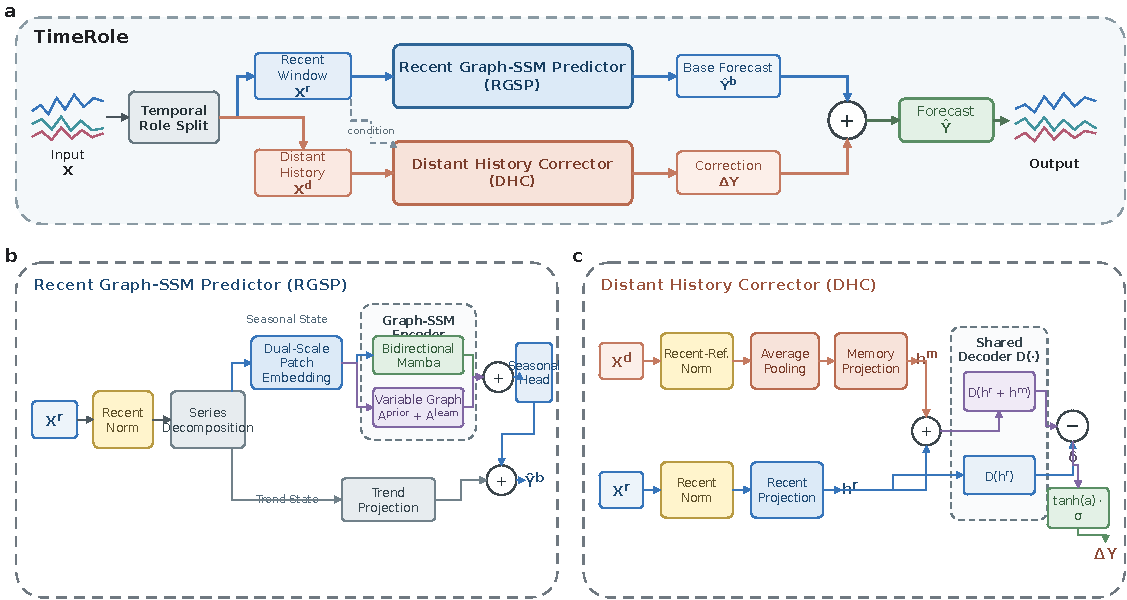
\includegraphics[width=\textwidth]{figures/Fig1_TimeRole_Architecture.pdf}
\caption{Overall architecture of TimeRole. \textbf{a} The input is partitioned by temporal position into a recent window and distant history. RGSP produces a base forecast at the original resolution, while DHC derives a conditional correction from the compressed distant history; the two outputs are combined to obtain the final forecast. \textbf{b} RGSP extracts recent dynamics and cross-variable dependencies through series decomposition, dual-scale patching, shared bidirectional Mamba encoding, and variable-graph propagation, and combines the resulting representation with a trend projection to form the base forecast. \textbf{c} DHC pools the distant history into memory tokens and forms a correction through paired outputs from a shared decoder conditioned on the recent state, followed by bounded variable-wise scaling.}
\label{fig:timerole-architecture}
\end{figure*}

\subsection{Recent graph-enhanced state-space predictor (RGSP)}

RGSP maps the recent window to a complete base forecast. As shown in Fig.~\ref{fig:timerole-architecture}(B), its forward process comprises series decomposition, dual-scale patch representation, bidirectional state-space encoding, variable-graph propagation, and forecast reconstruction.

\subsubsection{Recent decomposition and dual-scale representation}

Smooth evolution and local fluctuations exhibit different temporal patterns within the recent window. RGSP first applies a moving average to decompose the normalized recent sequence into trend and seasonal components \citep{Wu2021Autoformer,Zeng2023DLinear}:

\begin{equation}
\mathbf{T}^{r}=\operatorname{MA}(\widetilde{\mathbf{X}}^{r};w),\qquad
\mathbf{S}^{r}=\widetilde{\mathbf{X}}^{r}-\mathbf{T}^{r},
\label{eq:recent-decomposition}
\end{equation}

where \(w\) is the moving-average window size. The trend pathway preserves the smooth evolution of the recent window, whereas the seasonal pathway represents local deviations from this smooth trajectory. The trend component \(\mathbf{T}^{r}\) is projected along the temporal dimension to the prediction horizon using a variable-shared linear layer:

\begin{equation}
\widehat{\mathbf{Y}}^{\mathrm{tr}}_{:,n}
=\mathbf{W}_{\mathrm{tr}}\mathbf{T}^{r}_{:,n}
+\mathbf{b}_{\mathrm{tr}},
\qquad n=1,\ldots,N.
\label{eq:trend-projection}
\end{equation}

To represent local variations at different granularities within the same recent window, RGSP constructs coarse and fine patch grids from the seasonal component \(\mathbf{S}^{r}\). For scale \(s\in\{1,2\}\), let \(p_s\) and \(q_s\) denote the patch length and stride, respectively. After replicating \(q_s\) boundary values at the right end of the sequence, the number of patches is

\begin{equation}
J_s=\left\lfloor\frac{L_r+q_s-p_s}{q_s}\right\rfloor+1
\label{eq:patch-count}
\end{equation}

Let \(\mathcal{I}^{(s)}_j\) denote the temporal indices of the \(j\)-th patch. The token representation of variable \(n\) at this position is

\begin{equation}
\mathbf{z}^{(s)}_{n,j}
=\mathbf{W}^{(s)}_{p}\mathbf{S}^{r}_{\mathcal{I}^{(s)}_j,n}
+\mathbf{e}^{(s)}_{j}+\mathbf{v}_{n},
\qquad
\mathbf{z}^{(s)}_{n,j}\in\mathbb{R}^{d}.
\label{eq:patch-token}
\end{equation}

where \(\mathbf{W}^{(s)}_{p}\) is the patch projection matrix, \(\mathbf{e}^{(s)}_{j}\) is a sinusoidal positional encoding, and \(\mathbf{v}_{n}\) is a variable embedding shared across scales. Stacking all variables and patch positions gives the initial token tensor at scale \(s\):

\begin{equation}
\mathbf Z^{(s,0)}
=\operatorname{Stack}_{n,j}\!\left(\mathbf z^{(s)}_{n,j}\right)
\in\mathbb R^{N\times d\times J_s}.
\label{eq:scale-token-tensor}
\end{equation}

The coarse scale uses a larger \((p_s,q_s)\) to aggregate a wider temporal range, whereas the fine scale retains local variations with denser tokens. Both grids cover the same recent window rather than dividing it into two consecutive subintervals. They therefore produce tensors \(\mathbf Z^{(s,0)}\) with different shapes and are processed using the same state-space encoder parameters. The specific patch settings are provided in Section~4.1.

\subsubsection{Parameter-shared bidirectional state-space encoding}

The state-space branch models temporal dependencies along the patch sequence of each variable. The two scales share the same encoder parameters but are encoded independently; the final state of scale \(1\) is not used to initialize scale \(2\). Let \(\mathbf{Z}^{(s,\ell)}\in\mathbb{R}^{N\times d\times J_s}\) denote the input to layer \(\ell\) at scale \(s\). Omitting the batch dimension and dropout, the bidirectional Mamba layer is formulated as

\begin{equation}
\begin{aligned}
\mathbf{Q}^{(s,\ell)}
&=\mathbf{Z}^{(s,\ell)}
+\operatorname{Mamba}_{\rightarrow}
\!\left(\operatorname{LN}(\mathbf{Z}^{(s,\ell)})\right)\\
&\quad
+\operatorname{Rev}\!\left[
\operatorname{Mamba}_{\leftarrow}
\!\left(\operatorname{Rev}
\!\left[\operatorname{LN}(\mathbf{Z}^{(s,\ell)})\right]\right)
\right],
\end{aligned}
\label{eq:bidirectional-mamba}
\end{equation}

\begin{equation}
\mathbf{Z}^{(s,\ell+1)}
=\mathbf{Q}^{(s,\ell)}
+\operatorname{FFN}\!\left(\operatorname{LN}(\mathbf{Q}^{(s,\ell)})\right),
\qquad
\mathbf{U}^{(s)}=\operatorname{LN}(\mathbf{Z}^{(s,E)}),
\label{eq:mamba-ffn}
\end{equation}

where \(\operatorname{Rev}(\cdot)\) reverses the patch order, \(E\) is the number of encoder layers, and \(\mathbf{U}^{(s)}\) is the temporal state at scale \(s\). The forward scan propagates local evolution from earlier to later patches, whereas the backward scan aggregates context from patches near the forecast origin toward earlier positions. Together, they provide directionally complementary temporal representations on the same patch grid. Parameter sharing across scales applies a common state-transition mechanism to both temporal granularities without duplicating the encoder, while independent encoding preserves the sequence boundaries and token count of each scale.

\subsubsection{Variable-graph propagation and base-forecast reconstruction}

The temporal state \(\mathbf{U}^{(s)}\) describes the dynamics within each variable. RGSP further aggregates inter-variable dependencies through a parallel graph branch. A training-prior graph \(\mathbf{A}^{\mathrm{st}}\) is constructed using distance correlations computed over the training interval \citep{Szekely2007DistanceCorrelation}. For each variable, the \(K_g\) most strongly correlated neighbors and a self-connection are retained, followed by row normalization. In parallel, learnable node embeddings \(\mathbf{E}_{g}\) generate a global learned graph. The two types of relations are combined as

\begin{equation}
\mathbf{A}^{\mathrm{lrn}}
=\operatorname{softmax}(\mathbf{E}_{g}\mathbf{E}_{g}^{\mathsf T}),
\qquad
\mathbf{A}=\alpha\mathbf{A}^{\mathrm{st}}
+(1-\alpha)\mathbf{A}^{\mathrm{lrn}}.
\label{eq:graph-adjacency}
\end{equation}

where \(\alpha\in[0,1]\) controls the balance between the training-prior and globally learned relations. The graph \(\mathbf A^{\mathrm{st}}\) is constructed solely from the training interval and remains fixed during training, validation, and testing. By contrast, \(\mathbf A^{\mathrm{lrn}}\) is optimized jointly with the model parameters but shared across samples and temporal positions. The two graphs provide a data-derived adjacency prior and learnable global variable relations, respectively. At the \(j\)-th patch position of scale \(s\), let \(\overline{\mathbf{Z}}^{(s)}_{j}\in\mathbb{R}^{N\times d}\) denote the tokens of all variables obtained from Eq.~\eqref{eq:patch-token}. Graph propagation is computed as

\begin{equation}
\mathbf{G}^{(s)}_{j}
=\operatorname{GELU}
\!\left(\mathbf{A}\overline{\mathbf{Z}}^{(s)}_{j}\mathbf{W}_{\mathrm{in}}\right)
\mathbf{W}_{\mathrm{out}},
\qquad
\mathbf{H}^{(s)}_{j}=\mathbf{U}^{(s)}_{j}+\mathbf{G}^{(s)}_{j}.
\label{eq:graph-propagation}
\end{equation}

Here, \(\mathbf{W}_{\mathrm{in}}\) and \(\mathbf{W}_{\mathrm{out}}\) are feature projection matrices, with biases and dropout omitted for clarity. The tensors \(\mathbf{G}^{(s)}\) and \(\mathbf{H}^{(s)}\) denote the variable-graph state and the fused temporal-graph representation, respectively. The graph branch propagates information along the variable axis at each patch position, whereas the state-space branch propagates along the patch axis of each variable. These two axial flows are combined in \(\mathbf H^{(s)}\), such that each token contains both within-variable temporal dynamics and cross-variable information at the corresponding position.

Finally, RGSP concatenates the fused states from the two scales along the patch dimension, flattens the resulting representation for each variable, and generates the seasonal component through a prediction head:

\begin{equation}
\widehat{\mathbf{Y}}^{\mathrm{se}}
=\operatorname{Head}
\!\left(\mathbf{H}^{(1)}\mathbin{\Vert}_{p}\mathbf{H}^{(2)}\right),
\label{eq:seasonal-head}
\end{equation}

where \(\Vert_p\) denotes concatenation along the patch dimension. For each variable, the concatenated representation contains \(d(J_1+J_2)\) features, which the prediction head maps directly to \(H\) seasonal forecast values. All variables share the same form of output mapping while retaining their individual temporal-graph representations. The seasonal forecast is added to the trend forecast from Eq.~\eqref{eq:trend-projection}, and the statistics in Eq.~\eqref{eq:recent-statistics} restore the output to its original scale:

\begin{equation}
\begin{aligned}
\widehat{\mathbf{Y}}^{b,\mathrm{norm}}
&=\widehat{\mathbf{Y}}^{\mathrm{se}}
+\widehat{\mathbf{Y}}^{\mathrm{tr}},
\\
\widehat{\mathbf{Y}}^{b}_{:,n}
&=\sigma_n\widehat{\mathbf{Y}}^{b,\mathrm{norm}}_{:,n}+\mu_n.
\end{aligned}
\label{eq:base-forecast}
\end{equation}

The output \(\widehat{\mathbf{Y}}^{b}\) in Eq.~\eqref{eq:base-forecast} covers all \(H\) prediction steps and serves as the recent-window base forecast of TimeRole.

\subsection{Distant-history corrector (DHC)}

DHC converts distant history into a forecast correction conditioned on the recent state. As shown in Fig.~\ref{fig:timerole-architecture}(C), its main operations comprise history compression, state projection, paired decoding, and variable-wise injection. The module operates in parallel across variables without additional state-space scanning or graph propagation. A common set of projection and decoding parameters is applied to all variables, while variable-wise coefficients control the final correction strength.

\subsubsection{History compression and conditional states}

Distant history contains background variations spanning an extended temporal range. DHC applies non-overlapping average pooling with both width and stride equal to \(r\), compressing the \(L_d\) distant observations of each variable into \(K_m\) memory tokens:

\begin{equation}
\begin{aligned}
M_{n,k}
&=\frac{1}{r}\sum_{i=(k-1)r+1}^{kr}\widetilde X^d_{i,n},
\qquad k=1,\ldots,K_m,\\
\mathbf{M}
&=\operatorname{AvgPool}
\!\left((\widetilde{\mathbf{X}}^{d})^{\mathsf T};r\right)
\in\mathbb{R}^{N\times K_m},
\qquad K_m=\frac{L_d}{r}.
\end{aligned}
\label{eq:history-pooling}
\end{equation}

where \(r\) divides \(L_d\). Each memory token summarizes a consecutive, non-overlapping segment of distant observations. The resulting tokens preserve the original temporal order as a low-resolution historical trajectory and reduce the subsequent projection length from \(L_d\) to \(K_m\). For variable \(n\), DHC separately projects the recent window and compressed history into a \(d_h\)-dimensional conditioning space:

\begin{equation}
\mathbf{h}^{r}_{n}=\mathbf{W}_{r}\widetilde{\mathbf{x}}^{r}_{n},
\qquad
\mathbf{h}^{m}_{n}=\mathbf{W}_{m}\mathbf{m}_{n}.
\label{eq:dhc-states}
\end{equation}

Here, \(\widetilde{\mathbf{x}}^{r}_{n}\in\mathbb{R}^{L_r}\) and \(\mathbf{m}_{n}\in\mathbb{R}^{K_m}\) are the vectors of variable \(n\) in the recent window and compressed history, respectively; \(\mathbf{W}_{r}\in\mathbb{R}^{d_h\times L_r}\) and \(\mathbf{W}_{m}\in\mathbb{R}^{d_h\times K_m}\). The two bias-free linear mappings align temporal vectors of different lengths in the same conditioning space. The state \(\mathbf{h}^{r}_{n}\) represents the current predictive state, whereas \(\mathbf{h}^{m}_{n}\) represents the corresponding distant-history condition for the same variable. Their direct addition conditions the distant information on the current state without changing the output dimension.

\subsubsection{Paired decoding and variable-wise correction}

Within the conditioning space, DHC characterizes the forecast change induced by distant history through a pair of outputs. We define a shared bias-free decoder as \(D(\mathbf z)=\mathbf W_d\operatorname{GELU}(\mathbf z)\), where \(\mathbf{W}_{d}\in\mathbb{R}^{H\times d_h}\). For the same recent state, the decoder computes an output without and with the distant-history condition:

\begin{equation}
\begin{aligned}
\mathbf{y}^{-m}_{n}
&=D(\mathbf{h}^{r}_{n}),\qquad
\mathbf{y}^{+m}_{n}=D(\mathbf{h}^{r}_{n}+\mathbf{h}^{m}_{n}),
\\
\boldsymbol{\delta}_{n}
&=\mathbf{y}^{+m}_{n}-\mathbf{y}^{-m}_{n}\\
&=\mathbf W_d\!\left[
\operatorname{GELU}(\mathbf h_n^r+\mathbf h_n^m)
-\operatorname{GELU}(\mathbf h_n^r)
\right].
\end{aligned}
\label{eq:paired-decoding}
\end{equation}

The difference \(\boldsymbol{\delta}_{n}\in\mathbb{R}^{H}\) directly represents the forecast change produced by adding the distant condition \(\mathbf{h}^{m}_{n}\) to the recent state \(\mathbf{h}^{r}_{n}\). Both decoding operations use the same \(\mathbf W_d\) and differ only in whether the distant state is included. Consequently, their difference represents a conditional change rather than a discrepancy between two independent predictors. The shared decoder also places both outputs in the same forecast space, providing a consistent interface for step-wise correction.

Variables may respond to distant history with different strengths. DHC therefore assigns a learnable scalar \(a_n\) to each variable and obtains a variable-wise injection coefficient \(g_n\) through the hyperbolic tangent:

\begin{equation}
g_n=\tanh(a_n)\in(-1,1),\qquad
\Delta\mathbf{Y}_{:,n}
=g_n\sigma_n\boldsymbol{\delta}_{n}.
\label{eq:bounded-correction}
\end{equation}

The coefficient \(g_n\) is shared across all samples and prediction steps and determines the correction direction and relative strength for variable \(n\). A positive value preserves the direction of the decoded difference, a negative value permits an inverse adjustment, and its magnitude controls the injection ratio. The factor \(\sigma_n\) restores the output change from normalized space to the original scale. Combining this correction with Eq.~\eqref{eq:base-forecast} gives the final TimeRole prediction:

\begin{equation}
\widehat{\mathbf{Y}}_{:,n}
=\widehat{\mathbf{Y}}^{b}_{:,n}
+g_n\sigma_n\!\left[
D(\mathbf{h}^{r}_{n}+\mathbf{h}^{m}_{n})
-D(\mathbf{h}^{r}_{n})
\right].
\label{eq:timerole-output}
\end{equation}

Equation~\eqref{eq:timerole-output} combines the RGSP base forecast and the DHC distant-history conditional correction in the same output space, completing the TimeRole forecasting map.

\subsection{Joint optimization and computational complexity}

RGSP and DHC are trained jointly end to end using the final forecasting error. Given a batch size \(B\), the objective is the mean squared error between the predicted and ground-truth sequences:

\begin{equation}
\mathcal{L}_{\mathrm{MSE}}
=\frac{1}{BHN}
\sum_{b=1}^{B}\sum_{h=1}^{H}\sum_{n=1}^{N}
(\widehat{Y}_{b,h,n}-Y_{b,h,n})^2.
\label{eq:training-objective}
\end{equation}

The objective in Eq.~\eqref{eq:training-objective} is applied directly to the final output in Eq.~\eqref{eq:timerole-output}, allowing RGSP to learn the complete base forecast and DHC to learn a conditional correction from distant history. DHC introduces the recent-state projection \(\mathbf W_r\), history-state projection \(\mathbf W_m\), shared decoder \(\mathbf W_d\), and \(N\) variable-wise coefficients. Its parameter count is

\begin{equation}
P_{\mathrm{DHC}}=d_h(L_r+K_m+H)+N.
\label{eq:dhc-parameters}
\end{equation}

Relative to the recent backbone, the additional computational complexity of DHC is

\begin{equation}
\mathcal{O}\!\left(BNL_d+BNd_h(L_r+K_m+2H)\right).
\label{eq:dhc-complexity}
\end{equation}

The term \(BNL_d\) arises from distant-history pooling, and the remaining terms correspond to state projection and paired decoding. Because \(K_m=L_d/r\), subsequent mappings operate on the compressed memory length, whereas patch representation, state-space scanning, and graph propagation in RGSP process only the recent window of length \(L_r\). TimeRole can therefore extend its historical coverage by adjusting \(L_d\) and \(r\) without simultaneously increasing the sequence length processed by the recent backbone.

\section{Experiments}

\subsection{Experimental setup}

We evaluated TimeRole on five multivariate long-term forecasting benchmarks: ETTh1, ETTh2, ETTm1, ETTm2, and Weather \citep{Zhou2021Informer,Wu2021Autoformer,THUML2026TSLibDataset}. Their statistics are summarized in Table~\ref{tab:datasets}. All tasks followed the multivariate-input--multivariate-output setting with a unified input length of 336 and prediction horizons \(H\in\{96,192,336,720\}\). TimeRole partitioned each input into a recent window containing the last 96 observations and distant history containing the preceding 240 observations. The ETT datasets followed their public chronological splits, whereas Weather was divided into training, validation, and test sets at a ratio of 7:1:2. Forecasting accuracy was evaluated using mean squared error (MSE) and mean absolute error (MAE), with lower values indicating better performance.

\begin{table}[t]
\tablecaptionfont
\caption{Statistics of the five long-term forecasting datasets. The number of observations excludes the header, and the number of variables excludes the timestamp column.}
\label{tab:datasets}
\centering
\tablebodyfont
\setlength{\tabcolsep}{3pt}
\renewcommand{\arraystretch}{1.05}
\begin{tabular}{@{}lrrll@{}}
\toprule\noalign{}
Dataset & Variables & Observations & Frequency & Data split \\
\midrule\noalign{}
ETTh1 & 7 & 17,420 & 1 hour & Official ETT split \\
ETTh2 & 7 & 17,420 & 1 hour & Official ETT split \\
ETTm1 & 7 & 69,680 & 15 min & Official ETT split \\
ETTm2 & 7 & 69,680 & 15 min & Official ETT split \\
Weather & 21 & 52,696 & 10 min & 7:1:2 \\
\bottomrule\noalign{}
\end{tabular}
\end{table}

The main comparison included DLinear, PatchTST, iTransformer, TimeMixer, TimesNet, S-Mamba, and MSGNet \citep{Zeng2023DLinear,Nie2023PatchTST,Liu2024iTransformer,Wang2024TimeMixer,Wu2023TimesNet,Wang2025SMamba,Cai2024MSGNet}, covering linear, Transformer-based, multiscale, state-space, and variable-graph forecasting approaches. The main comparison, RGSP-96 control, and cross-backbone transfer experiments used the same data splits, evaluation scripts, and validation-based checkpoint selection rule. Each experiment was run independently with random seeds \(\{2021,2022,2023\}\).

TimeRole was optimized using Adam with an initial learning rate of \(5\times10^{-4}\), a batch size of 32, and a dropout rate of 0.1. Training was limited to 100 epochs and stopped early when the validation MSE did not improve for six consecutive epochs. All experiments were conducted using PyTorch 2.5.1 and CUDA 12.1 on a single NVIDIA GeForce RTX 4090 GPU.

\subsection{Overall forecasting performance}

Table~\ref{tab:main-results} reports the three-seed mean test performance of eight methods on five datasets and four prediction horizons. Across the 20 dataset--horizon tasks, TimeRole achieved the lowest MSE and MAE in 11 tasks each, with an additional three second-best MSE values and five second-best MAE values. Its task-level average ranks were 1.95 for MSE and 1.75 for MAE, the lowest among all compared methods.

Across prediction horizons of 96, 192, 336, and 720, TimeRole obtained the lowest MSE in 3, 3, 3, and 2 tasks, respectively; the distribution was identical for MAE. At the dataset level, it achieved the lowest MSE and MAE at all four horizons on Weather and at horizons 96--336 on ETTh2. It also attained the lowest values for both metrics at horizons 96 and 720 on ETTh1, the lowest MAE at horizon 336 on ETTh1, and the lowest MSE at horizons 192 and 336 on ETTm1. These results show that TimeRole remained competitive across different sampling frequencies and prediction horizons.

The strongest baseline varied across datasets and prediction horizons, whereas the best results of TimeRole were distributed across multiple datasets and all four horizons. For a stricter comparison, we constructed a per-task oracle that selected the best-performing baseline for each task and therefore assumed prior knowledge of the optimal model. Relative to this oracle, TimeRole had a 0.376\% higher macro-average MSE and a 0.059\% lower macro-average MAE across the 20 tasks. Thus, a single TimeRole architecture achieved overall accuracy comparable to per-task baseline selection without requiring dataset- or horizon-specific model choices.

\begin{table*}[!t]
\begingroup
\tablecaptionfont
\caption{Quantitative comparison on five datasets with an input length of 336 and prediction horizons of 96, 192, 336, and 720. Values are test-set means over three random seeds. Best results are shown in bold and second-best results are underlined. Lower MSE and MAE values indicate better performance.}
\label{tab:main-results}
\centering
\wideresulttablefont
\setlength{\tabcolsep}{0.5pt}
\renewcommand{\arraystretch}{1.08}
\begin{tabular*}{\textwidth}{@{\extracolsep{\fill}}ll*{16}{c}@{}}
\toprule
\multirow{2}{*}{Dataset} & \multirow{2}{*}{\(H\)} & \multicolumn{2}{c}{TimeRole} & \multicolumn{2}{c}{S-Mamba} & \multicolumn{2}{c}{iTransformer} & \multicolumn{2}{c}{TimeMixer} & \multicolumn{2}{c}{MSGNet} & \multicolumn{2}{c}{PatchTST} & \multicolumn{2}{c}{TimesNet} & \multicolumn{2}{c}{DLinear} \\
\cmidrule(lr){3-4}\cmidrule(lr){5-6}\cmidrule(lr){7-8}\cmidrule(lr){9-10}\cmidrule(lr){11-12}\cmidrule(lr){13-14}\cmidrule(lr){15-16}\cmidrule(lr){17-18}
& & MSE & MAE & MSE & MAE & MSE & MAE & MSE & MAE & MSE & MAE & MSE & MAE & MSE & MAE & MSE & MAE \\
\midrule
ETTh1 & 96 & \textbf{0.369} & \textbf{0.398} & 0.397 & 0.417 & 0.399 & 0.417 & 0.389 & 0.408 & 0.422 & 0.441 & 0.399 & 0.420 & 0.437 & 0.450 & \underline{0.375} & \underline{0.399} \\
 & 192 & \underline{0.415} & \underline{0.426} & 0.434 & 0.441 & 0.442 & 0.446 & 0.437 & 0.438 & 0.455 & 0.465 & 0.462 & 0.461 & 0.466 & 0.468 & \textbf{0.408} & \textbf{0.419} \\
 & 336 & \underline{0.449} & \textbf{0.443} & 0.452 & 0.455 & 0.464 & 0.462 & 0.474 & 0.466 & 0.481 & 0.479 & 0.528 & 0.503 & 0.519 & 0.502 & \textbf{0.439} & \underline{0.445} \\
 & 720 & \textbf{0.454} & \textbf{0.458} & 0.511 & 0.509 & 0.506 & 0.507 & 0.726 & 0.593 & 0.524 & 0.515 & 0.657 & 0.571 & 0.589 & 0.537 & \underline{0.471} & \underline{0.492} \\
ETTh2 & 96 & \textbf{0.283} & \textbf{0.343} & 0.301 & 0.358 & 0.302 & 0.359 & \underline{0.283} & \underline{0.348} & 0.369 & 0.414 & 0.323 & 0.372 & 0.363 & 0.414 & 0.303 & 0.367 \\
 & 192 & \textbf{0.344} & \textbf{0.387} & 0.366 & \underline{0.398} & 0.388 & 0.410 & \underline{0.361} & 0.400 & 0.398 & 0.429 & 0.389 & 0.421 & 0.407 & 0.439 & 0.397 & 0.429 \\
 & 336 & \textbf{0.375} & \textbf{0.413} & 0.394 & 0.420 & 0.420 & 0.434 & \underline{0.383} & \underline{0.416} & 0.400 & 0.437 & 0.428 & 0.444 & 0.407 & 0.443 & 0.482 & 0.482 \\
 & 720 & 0.449 & 0.462 & \textbf{0.418} & \textbf{0.445} & \underline{0.424} & \underline{0.447} & 0.425 & 0.451 & 0.444 & 0.464 & 0.463 & 0.475 & 0.426 & 0.456 & 0.751 & 0.615 \\
ETTm1 & 96 & \underline{0.298} & 0.352 & 0.301 & 0.356 & 0.305 & 0.358 & \textbf{0.292} & \underline{0.347} & 0.309 & 0.363 & 0.317 & 0.366 & 0.324 & 0.370 & 0.300 & \textbf{0.344} \\
 & 192 & \textbf{0.333} & \underline{0.374} & 0.344 & 0.383 & 0.344 & 0.382 & 0.339 & 0.375 & 0.356 & 0.393 & 0.352 & 0.386 & 0.382 & 0.399 & \underline{0.334} & \textbf{0.364} \\
 & 336 & \textbf{0.368} & \underline{0.395} & 0.378 & 0.403 & 0.380 & 0.403 & 0.405 & 0.415 & 0.389 & 0.412 & 0.395 & 0.418 & 0.401 & 0.414 & \underline{0.370} & \textbf{0.387} \\
 & 720 & 0.429 & 0.429 & 0.436 & 0.437 & 0.440 & 0.437 & \underline{0.428} & \underline{0.426} & 0.444 & 0.448 & 0.451 & 0.452 & 0.478 & 0.459 & \textbf{0.426} & \textbf{0.422} \\
ETTm2 & 96 & 0.176 & 0.264 & 0.179 & 0.270 & 0.175 & 0.266 & \underline{0.173} & \underline{0.262} & 0.188 & 0.273 & 0.182 & 0.272 & 0.197 & 0.279 & \textbf{0.167} & \textbf{0.262} \\
 & 192 & 0.231 & \textbf{0.300} & 0.237 & 0.310 & 0.243 & 0.312 & \underline{0.230} & \underline{0.301} & 0.242 & 0.311 & 0.236 & 0.309 & 0.240 & 0.311 & \textbf{0.229} & 0.309 \\
 & 336 & 0.285 & \underline{0.336} & \underline{0.284} & 0.339 & 0.299 & 0.348 & \textbf{0.280} & \textbf{0.335} & 0.302 & 0.349 & 0.308 & 0.357 & 0.302 & 0.351 & 0.302 & 0.363 \\
 & 720 & 0.376 & \underline{0.392} & \underline{0.375} & 0.394 & 0.377 & 0.395 & \textbf{0.364} & \textbf{0.387} & 0.402 & 0.406 & 0.395 & 0.408 & 0.436 & 0.421 & 0.421 & 0.439 \\
Weather & 96 & \textbf{0.146} & \textbf{0.197} & 0.157 & 0.206 & 0.163 & 0.212 & \underline{0.148} & \underline{0.198} & 0.162 & 0.218 & 0.156 & 0.206 & 0.166 & 0.225 & 0.175 & 0.237 \\
 & 192 & \textbf{0.188} & \textbf{0.237} & 0.204 & 0.252 & 0.205 & 0.250 & \underline{0.192} & \underline{0.241} & 0.211 & 0.260 & 0.201 & 0.247 & 0.215 & 0.266 & 0.216 & 0.274 \\
 & 336 & \textbf{0.242} & \textbf{0.278} & 0.256 & 0.288 & 0.257 & 0.290 & \underline{0.242} & \underline{0.281} & 0.261 & 0.294 & 0.257 & 0.290 & 0.272 & 0.307 & 0.262 & 0.314 \\
 & 720 & \textbf{0.318} & \textbf{0.332} & 0.326 & 0.339 & 0.331 & 0.340 & \underline{0.319} & \underline{0.333} & 0.370 & 0.362 & 0.330 & 0.340 & 0.348 & 0.355 & 0.326 & 0.366 \\
\bottomrule
\end{tabular*}
\endgroup
\end{table*}

Fig.~\ref{fig:forecast-profiles} compares the forecasts of the eight models on the same ETTh2 test window, showing their reconstruction of phase, amplitude, and local patterns. The sample origin was selected according to the total variation of the ground-truth target sequence without using model errors.

\begin{figure*}[t]
\centering
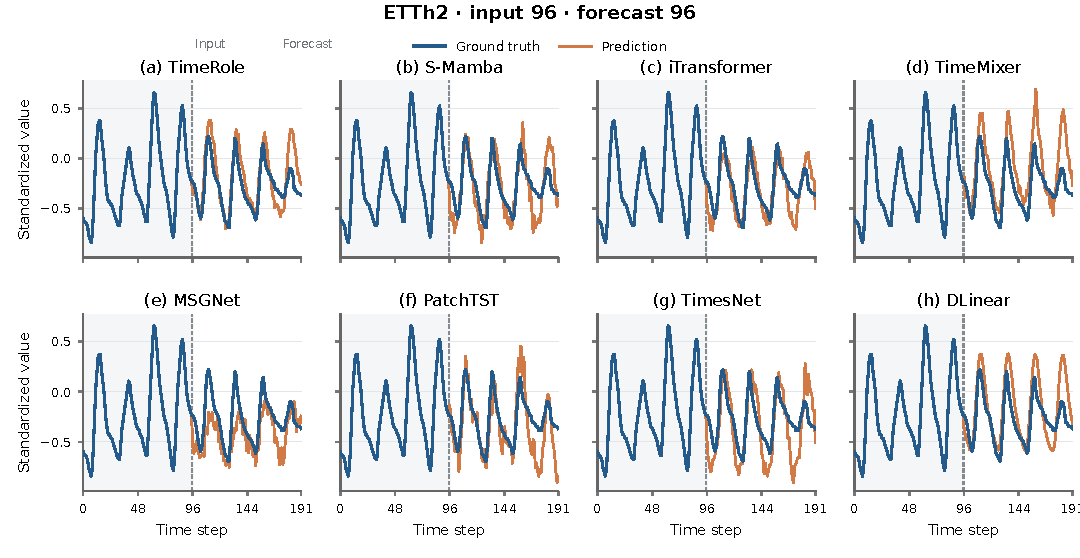
\includegraphics[width=\textwidth]{figures/Fig3_Model_Comparison_v2.pdf}
\caption{Normalized forecasting example for eight models on ETTh2 with both input and prediction lengths set to 96. The shaded region denotes the shared input, the dashed line marks the forecast origin, and the blue and orange curves represent the ground truth and model prediction, respectively. The test origin was selected using the median total variation of the 720-step ground-truth targets without reference to model error.}
\label{fig:forecast-profiles}
\end{figure*}

\subsection{Attributing the contribution of history-role differentiation}

To isolate the contribution of distant-history correction, Table~\ref{tab:recent96-comparison} compares TimeRole with the internal RGSP-96 variant under the same recent forecasting pathway, while Fig.~\ref{fig:timerole-evidence}a shows the corresponding seed-wise gains. RGSP-96 retains only RGSP and uses the final 96 observations as input, without DHC. TimeRole uses the same recent backbone, optimization settings, and checkpoint selection rule, while additionally compressing the preceding 240 observations to generate a conditional correction. The two models therefore differ only in whether DHC is included.

\begin{figure*}[t]
\centering
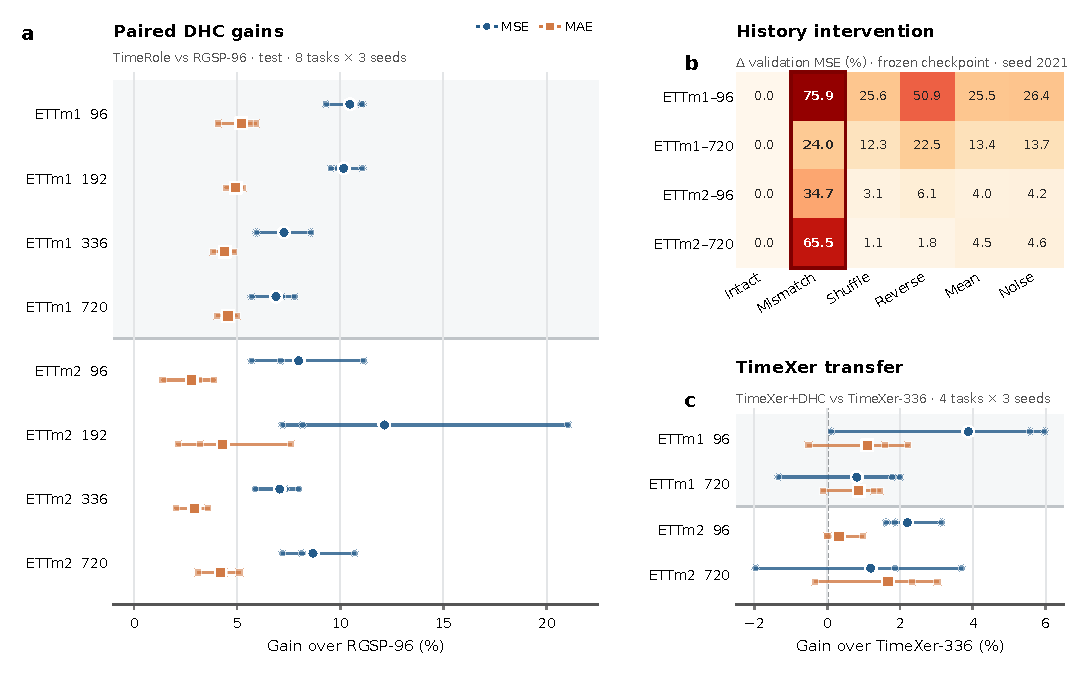
\includegraphics[width=\textwidth]{figures/Fig2_TimeRole_Evidence_v2.pdf}
\caption{Complementary evidence for distant-history conditional correction. \textbf{a} Seed-wise test gains of TimeRole over RGSP-96. \textbf{b} Changes in validation MSE induced by distant-history interventions at the frozen checkpoint for seed 2021. \textbf{c} Seed-wise test gains of TimeXer+DHC over the direct long-input TimeXer configuration. Positive values in \textbf{a,c} indicate error reductions. Small markers, large markers, and horizontal lines denote paired seeds, task means, and observed ranges, respectively; the horizontal lines are not confidence intervals.}
\label{fig:timerole-evidence}
\end{figure*}

\begin{table}[!t]
\tablecaptionfont
\caption{Comparison between TimeRole and RGSP-96 on ETTm1 and ETTm2. Values are test-set means $\pm$ sample standard deviations over three random seeds. Best results are shown in bold and second-best results are underlined. Lower MSE and MAE values indicate better performance.}
\label{tab:recent96-comparison}
\centering
\tablebodyfont
\fontsize{7.7}{8.9}\selectfont
\setlength{\tabcolsep}{3pt}
\renewcommand{\arraystretch}{1.08}
\begin{tabular*}{\columnwidth}{@{\extracolsep{\fill}}lllrr@{}}
\toprule\noalign{}
Dataset & \(H\) & Method & MSE & MAE \\
\midrule\noalign{}
ETTm1 & 96 & TimeRole & \textbf{0.298±0.003} & \textbf{0.352±0.003} \\
& & RGSP-96 & \underline{0.333±0.003} & \underline{0.371±0.003} \\
& 192 & TimeRole & \textbf{0.333±0.001} & \textbf{0.374±0.001} \\
& & RGSP-96 & \underline{0.371±0.004} & \underline{0.393±0.002} \\
& 336 & TimeRole & \textbf{0.368±0.002} & \textbf{0.395±0.001} \\
& & RGSP-96 & \underline{0.397±0.006} & \underline{0.413±0.003} \\
& 720 & TimeRole & \textbf{0.429±0.004} & \textbf{0.429±0.002} \\
& & RGSP-96 & \underline{0.460±0.003} & \underline{0.449±0.002} \\
\midrule
ETTm2 & 96 & TimeRole & \textbf{0.176±0.004} & \textbf{0.264±0.003} \\
& & RGSP-96 & \underline{0.191±0.010} & \underline{0.272±0.007} \\
& 192 & TimeRole & \textbf{0.231±0.009} & \textbf{0.300±0.008} \\
& & RGSP-96 & \underline{0.265±0.035} & \underline{0.314±0.018} \\
& 336 & TimeRole & \textbf{0.285±0.005} & \textbf{0.336±0.005} \\
& & RGSP-96 & \underline{0.307±0.003} & \underline{0.346±0.003} \\
& 720 & TimeRole & \textbf{0.375±0.001} & \textbf{0.392±0.003} \\
& & RGSP-96 & \underline{0.411±0.009} & \underline{0.409±0.007} \\
\bottomrule\noalign{}
\end{tabular*}
\end{table}

As shown in Table~\ref{tab:recent96-comparison}, TimeRole reduced both the mean MSE and MAE in all eight ETTm1 and ETTm2 tasks. Relative to RGSP-96, the MSE reductions ranged from 6.884\% to 12.824\%, with a task-level macro-average reduction of 8.828\%. The corresponding MAE reductions ranged from 2.824\% to 5.203\%, with a macro-average reduction of 4.162\%. Across the 24 seed-wise pairs formed by three independent runs, TimeRole achieved lower MSE and MAE in every comparison. This pattern covered all four prediction horizons of 96, 192, 336, and 720.

With the recent predictor and training protocol held fixed, introducing compressed distant history consistently improved the base forecast. The observed gains show that the additional historical range contributed useful information through the conditional correction pathway.

\subsection{Design and mechanism analysis}

\subsubsection{System-level component sensitivity}

Table~\ref{tab:core-component-sensitivity} compares the complete TimeRole model with three removal variants. RGSP-96 removes DHC, whereas w/o Graph and w/o Patch disable variable-graph propagation and patch representation in RGSP, respectively. The experiments cover four prediction horizons on ETTm1, ETTm2, and Weather, with each configuration retrained using three random seeds. To summarize the cross-task pattern, the table reports the task-level macro-average error change of each variant relative to the complete model and counts the tasks in which the complete model achieves a lower error.

\begin{table*}[t]
\tablecaptionfont
\caption{System-level component sensitivity of TimeRole across four prediction horizons on ETTm1, ETTm2, and Weather. Error changes are task-level macro averages relative to the complete model after removing the corresponding component; positive values indicate increased errors. Wins count the tasks in which the complete model achieves lower MSE/MAE.}
\label{tab:core-component-sensitivity}
\centering
\tablebodyfont
\setlength{\tabcolsep}{4pt}
\renewcommand{\arraystretch}{1.08}
\begin{tabular*}{\textwidth}{@{\extracolsep{\fill}}lrrrrr@{}}
\toprule\noalign{}
\multirow{2}{*}{Variant} & \multicolumn{4}{c}{Error change (MSE/MAE)} & \multirow{2}{*}{Wins} \\
\cmidrule(lr){2-5}
& ETTm1 & ETTm2 & Weather & Overall & \\
\midrule\noalign{}
RGSP-96 & +9.562/+5.012 & +10.156/+3.729 & +9.489/+5.503 & +9.736/+4.748 & 12/12 \\
w/o Graph & -0.324/-0.267 & +1.134/+1.029 & +0.161/+0.173 & +0.324/+0.312 & 7/8 \\
w/o Patch & +1.195/+0.523 & +2.672/+1.375 & -0.457/-0.356 & +1.137/+0.514 & 7/7 \\
\bottomrule\noalign{}
\end{tabular*}
\end{table*}

Removing DHC increased the macro-average MSE by at least 9.489\% on each dataset and increased the overall MSE and MAE across the 12 tasks by 9.736\% and 4.748\%, respectively. The complete model achieved lower values for both metrics in every task. DHC was therefore the most consistent source of improvement among the evaluated system components, in agreement with the RGSP-96 comparison in Section~4.3.

The effects of Graph and Patch in the recent pathway were more dataset dependent. Removing them increased the overall MSE by 0.324\% and 1.137\%, respectively, with the complete model winning 7 of 12 tasks in MSE for both comparisons. Graph contributed positively on ETTm2 and Weather, whereas Patch had a clearer effect on ETTm1 and ETTm2. Thus, variable-graph propagation and patch representation both improved average cross-task performance, although their gains were concentrated in particular datasets and horizons.

All variants were retrained jointly with DHC, so Table~\ref{tab:core-component-sensitivity} reflects the performance of the complete system after each component change. The results distinguish the stable contribution of distant-history correction from the dataset- and horizon-dependent effects of components in the recent pathway.

\subsubsection{DHC design choices}

Table~\ref{tab:design-choices} compares the complete TimeRole model with three internal variants to examine how distant information is conditioned. Concat directly concatenates the recent state and distant memory before producing the forecast, thereby comparing paired decoding with direct fusion. NoDiff removes the difference between the two decoded outputs, and GlobalGate replaces the variable-wise correction coefficients with a global coefficient shared across variables. The experiments cover the 96- and 720-step tasks on ETTm1 and ETTm2 and are repeated with three random seeds.

The complete TimeRole model achieved the lowest MSE and MAE on ETTm1-96 and ETTm1-720, as well as the lowest MAE on ETTm2-720. In seed-wise paired comparisons, TimeRole recorded 9/12, 9/12, and 7/12 MSE wins over Concat, NoDiff, and GlobalGate, corresponding to macro-average improvements of 0.743\%, 0.912\%, and 0.189\%, respectively. NoDiff attained the lowest MSE on ETTm2-96, whereas GlobalGate attained the lowest MSE on ETTm2-720, indicating that alternative conditioning forms can be better suited to individual tasks.

\begin{table}[t]
\tablecaptionfont
\caption{DHC design choices in TimeRole. Paired differencing, direct concatenation, no differencing, and global gating are compared on the 96- and 720-step tasks of ETTm1 and ETTm2. Values are test-set means $\pm$ sample standard deviations over three random seeds. Best results are shown in bold and second-best results are underlined.}
\label{tab:design-choices}
\centering
\tablebodyfont
\setlength{\tabcolsep}{3pt}
\renewcommand{\arraystretch}{1.08}
\begin{tabular*}{\columnwidth}{@{\extracolsep{\fill}}llrrr@{}}
\toprule\noalign{}
Dataset & \(H\) & Method & MSE & MAE \\
\midrule\noalign{}
ETTm1 & 96 & TimeRole & \textbf{0.298±0.003} & \textbf{0.352±0.003} \\
& & RGSP-96 & 0.333±0.003 & 0.371±0.003 \\
& & Concat & 0.303±0.004 & 0.354±0.001 \\
& & NoDiff & 0.307±0.004 & 0.356±0.001 \\
& & GlobalGate & \underline{0.300±0.003} & \underline{0.353±0.002} \\
\addlinespace[1pt]
& 720 & TimeRole & \textbf{0.429±0.004} & \textbf{0.429±0.002} \\
& & RGSP-96 & 0.460±0.003 & 0.449±0.002 \\
& & Concat & 0.434±0.002 & \underline{0.430±0.001} \\
& & NoDiff & 0.433±0.002 & 0.430±0.001 \\
& & GlobalGate & \underline{0.432±0.003} & 0.431±0.001 \\
\midrule
ETTm2 & 96 & TimeRole & 0.176±0.004 & 0.264±0.003 \\
& & RGSP-96 & 0.191±0.010 & 0.272±0.007 \\
& & Concat & 0.176±0.005 & 0.265±0.004 \\
& & NoDiff & \textbf{0.175±0.003} & \underline{0.264±0.003} \\
& & GlobalGate & \underline{0.175±0.004} & \textbf{0.264±0.003} \\
\addlinespace[1pt]
& 720 & TimeRole & \underline{0.375±0.001} & \textbf{0.392±0.003} \\
& & RGSP-96 & 0.411±0.009 & 0.409±0.007 \\
& & Concat & 0.377±0.002 & 0.393±0.003 \\
& & NoDiff & 0.376±0.001 & 0.393±0.003 \\
& & GlobalGate & \textbf{0.374±0.000} & \underline{0.392±0.003} \\
\bottomrule\noalign{}
\end{tabular*}
\end{table}

Overall, the differences among the internal DHC variants were smaller than the gains of TimeRole over RGSP-96. Paired differencing with variable-wise correction provided a balanced MSE--MAE profile across the four endpoint tasks, while the local advantages of alternative variants on ETTm2 suggest that the correction form could be further adapted to sequence characteristics.

\subsubsection{Distant-history interventions}

Frozen-checkpoint interventions were used to examine the response of DHC to distant-history content. The final 96-point recent window and all model parameters were held fixed, and only the preceding 240 observations provided to DHC were modified at inference time. Sample mismatch changed the correspondence between the distant history and the current sample; temporal shuffling and reversal altered the internal order of the history; and mean and noise replacement removed the observed trajectory while retaining its basic numerical scale. The resulting error changes quantify the model's sensitivity to different aspects of distant information.

Figure~\ref{fig:timerole-evidence}b and Table~\ref{tab:history-intervention} show that all 20 interventions increased validation MSE, with an average increase of 20.992\%. Sample mismatch produced the largest error increase in each of the four tasks, ranging from 24.05\% to 75.91\%. Mean and noise replacement also degraded performance in every task. These observations show that the correction produced by DHC depends on both the distant-history content and its correspondence with the current sample.

The response to historical structure differed across datasets. On ETTm1, temporal shuffling increased MSE by 25.60\% at horizon 96 and 12.29\% at horizon 720, while temporal reversal increased it by 50.87\% and 22.51\%, respectively. ETTm2 was less sensitive to these order interventions, but sample mismatch still increased MSE by 34.65\% and 65.48\% at the two horizons. This contrast suggests that the ETTm1 forecasts relied more strongly on distant-history order, whereas ETTm2 under the present configuration relied more on sample consistency between the distant history and recent window.

\begin{table}[t]
\tablecaptionfont
\caption{Distant-history interventions at a frozen checkpoint. Model parameters and the recent window are held fixed, and only the distant history supplied to DHC is replaced or reordered. Values are relative increases in validation MSE for random seed 2021; positive values indicate degradation relative to the intact history.}
\label{tab:history-intervention}
\centering
\tablebodyfont
\setlength{\tabcolsep}{1.5pt}
\renewcommand{\arraystretch}{1.08}
\begin{tabular}{@{}llccccc@{}}
\toprule\noalign{}
Dataset & \(H\) & Mismatch & Shuffle & Reverse & Mean & Noise \\
\midrule\noalign{}
ETTm1 & 96 & +75.91\% & +25.60\% & +50.87\% & +25.49\% & +26.39\% \\
& 720 & +24.05\% & +12.29\% & +22.51\% & +13.41\% & +13.72\% \\
ETTm2 & 96 & +34.65\% & +3.13\% & +6.05\% & +4.04\% & +4.16\% \\
& 720 & +65.48\% & +1.14\% & +1.80\% & +4.54\% & +4.61\% \\
\bottomrule\noalign{}
\end{tabular}
\end{table}

\subsubsection{History-role boundary and compression sensitivity}

To evaluate TimeRole under different allocations of historical range and resolution, we varied the total history length, recent-window length, and DHC pooling width. The total-history experiment covers the 96- and 720-step tasks on ETTm1, ETTm2, and Weather, using input lengths of 192, 336, 720, and 960 while fixing the recent window at 96 and the pooling width at 16. The boundary and compression experiments fix the total history at 336 on ETTm1 and ETTm2 and compare recent-window lengths of 48, 96, and 192 and pooling widths of 8, 16, and 24. Each configuration was independently trained with three random seeds; checkpoints were selected by validation MSE and test-set means were reported. The unified main setting, comprising a 336-point total history, a 96-point recent window, and a pooling width of 16, serves as the reference.

\begin{figure*}[t]
\centering
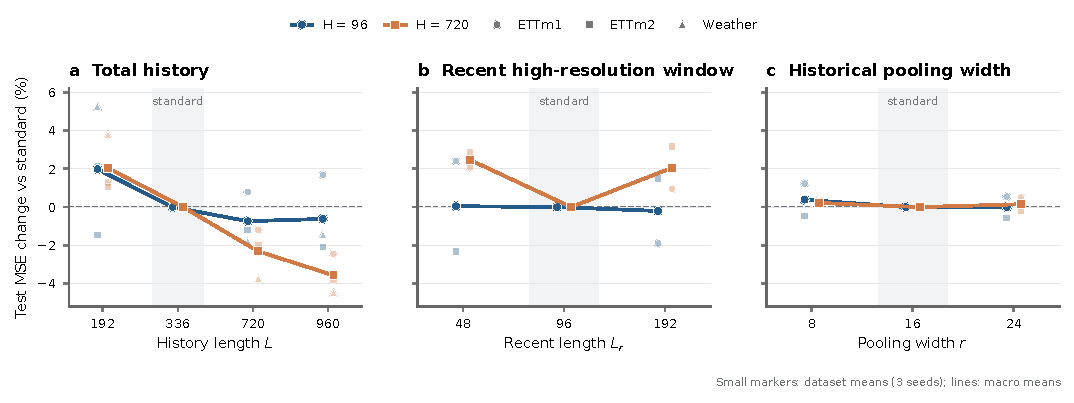
\includegraphics[width=\textwidth]{figures/Fig4_History_Sensitivity_v1.pdf}
\caption{Sensitivity of TimeRole to historical range and resolution allocation. \textbf{a--c} vary the total history length, recent high-resolution window, and DHC pooling width, respectively. The vertical axis shows the change in test MSE relative to the unified setting (total history 336, recent window 96, and pooling width 16). Light markers denote three-seed means for individual datasets, and connected markers denote task-level macro averages at the same prediction horizon.}
\label{fig:history-sensitivity}
\end{figure*}

Expanding the total historical range yielded more consistent gains for long-horizon forecasting. Relative to a 336-point history, histories of 720 and 960 points reduced the macro-average test MSE across the six dataset--horizon tasks by 1.526\% and 2.093\%, respectively. For the 720-step forecasts, the average reductions increased to 2.314\% and 3.566\%, and the 960-point history achieved lower MSE on ETTm1, ETTm2, and Weather. Short-horizon tasks showed different preferences: the lowest MSE on ETTm1, ETTm2, and Weather occurred at 336, 960, and 720 points, respectively. Meanwhile, the macro-average MAE change relative to 336 points remained within 0.622\% for every history length, indicating a stronger effect on squared error. Extending the history from 336 to 960 points increased the parameter count by no more than 0.13\%, allowing DHC to expand distant coverage without lengthening the sequence processed by the recent backbone.

The recent-window length exposes the capacity trade-off between high-resolution modeling and distant-history compression. Relative to a 96-point recent window, shortening the window to 48 points increased the four-task macro-average test MSE by 1.254\% while reducing the average parameter count by 48.5\%. Extending it to 192 points increased the average parameter count by 97.0\% and the macro-average MSE by 0.928\%. The 96-point window achieved the lowest MSE among the three settings on both 720-step tasks, whereas the lowest MSE for 96-step forecasting occurred with 192 points on ETTm1 and 48 points on ETTm2. Increasing the recent high-resolution pathway therefore provided no consistent benefit, and the 96-point window offered a balanced allocation between recent-state resolution and model capacity over the evaluated tasks.

DHC was comparatively insensitive to the evaluated pooling widths. Relative to a width of 16, widths of 8 and 24 changed the four-task macro-average test MSE by +0.301\% and +0.070\%, respectively, while both macro-average MAE changes remained below 0.21\%. ETTm1 generally favored a width of 16, whereas some ETTm2 tasks performed slightly better at 24, reflecting differences in the preferred resolution of distant memory. Taken together, the total-history, recent-window, and pooling-width results identify a 336-point total history, a 96-point recent window, and a pooling width of 16 as a stable configuration under the unified protocol. Longer distant coverage benefited long-horizon forecasting, whereas directly enlarging the recent window substantially increased model capacity.

\subsection{Generalizability and practical cost}

\subsubsection{Transfer across forecasting backbones}

To determine whether recent--distant role differentiation depends on the graph and state-space structure of RGSP, we integrated DHC with TimeXer \citep{Wang2024TimeXer}. TimeXer organizes its input using patch self-attention and variate cross-attention, providing a forecasting pathway distinct from RGSP. The cross-backbone experiments consider three history-routing strategies: TimeXer-Recent96 uses only the final 96 observations; TimeXer+DHC sends the final 96 observations to TimeXer and compresses the preceding 240 observations into a conditional correction; and TimeXer-336 directly processes all 336 observations using the original TimeXer. Every dataset--horizon setting uses the same data splits, model preset, optimization settings, and validation-based checkpoint rule and is run with three random seeds. The difference between TimeXer+DHC and TimeXer-Recent96 quantifies the incremental effect of distant-history correction, whereas the comparison with TimeXer-336 contrasts role differentiation with direct long input.

As shown in Fig.~\ref{fig:timerole-evidence}c and Table~\ref{tab:backbone-transfer}, TimeXer+DHC achieved lower three-seed mean MSE and MAE than TimeXer-336 on all 96- and 720-step endpoint tasks of ETTm1 and ETTm2. Across these four tasks, the MSE reductions ranged from 0.82\% to 3.88\% and the MAE reductions from 0.33\% to 1.67\%, with task-level macro-average reductions of 2.02\% and 0.99\%, respectively. In seed-wise comparisons, TimeXer+DHC recorded 10/12 MSE wins and 8/12 MAE wins.

\begin{table}[t]
\tablecaptionfont
\caption{Comparison of TimeXer-336 and TimeXer+DHC on ETTm1 and ETTm2. Both methods access the same aligned 336-point history. Values are test-set means $\pm$ sample standard deviations over three random seeds, with checkpoints selected by validation MSE.}
\label{tab:backbone-transfer}
\centering
\tablebodyfont
\setlength{\tabcolsep}{3pt}
\renewcommand{\arraystretch}{1.08}
\begin{tabular*}{\columnwidth}{@{\extracolsep{\fill}}lllrr@{}}
\toprule\noalign{}
Dataset & \(H\) & Method & MSE & MAE \\
\midrule\noalign{}
ETTm1 & 96 & TimeXer+DHC & \textbf{0.298$\pm$0.002} & \textbf{0.350$\pm$0.001} \\
& & TimeXer-336 & \underline{0.310$\pm$0.010} & \underline{0.354$\pm$0.004} \\
& 720 & TimeXer+DHC & \textbf{0.431$\pm$0.002} & \textbf{0.429$\pm$0.001} \\
& & TimeXer-336 & \underline{0.435$\pm$0.006} & \underline{0.433$\pm$0.003} \\
\midrule
ETTm2 & 96 & TimeXer+DHC & \textbf{0.165$\pm$0.002} & \textbf{0.254$\pm$0.002} \\
& & TimeXer-336 & \underline{0.169$\pm$0.001} & \underline{0.255$\pm$0.001} \\
& 720 & TimeXer+DHC & \textbf{0.375$\pm$0.003} & \textbf{0.390$\pm$0.004} \\
& & TimeXer-336 & \underline{0.380$\pm$0.010} & \underline{0.397$\pm$0.008} \\
\bottomrule\noalign{}
\end{tabular*}
\end{table}

Table~\ref{tab:backbone-transfer-etth} extends the transfer evaluation to all four horizons on ETTh1 and ETTh2 and includes TimeXer-Recent96 to separate the effect of distant-history correction from those of a short recent input and a direct long input. Relative to TimeXer-336, TimeXer+DHC achieved lower mean MSE and MAE simultaneously in 7 of 8 tasks, with task-level macro-average reductions of 7.33\% and 5.11\%, respectively. Relative to TimeXer-Recent96, its mean MSE was lower in 7/8 tasks, with a macro-average reduction of 3.12\%, while its mean MAE was lower in 4/8 tasks, with a macro-average reduction of 0.71\%. TimeXer+DHC achieved the lowest mean values for both metrics on the 192- and 336-step tasks of ETTh1 and ETTh2, showing the most consistent gains at intermediate horizons.

\begin{table*}[t]
\tablecaptionfont
\caption{Comparison of three TimeXer history-routing strategies on ETTh1 and ETTh2. TimeXer-Recent96 uses only the final 96 observations, TimeXer+DHC corrects the recent forecast using the preceding 240 observations, and TimeXer-336 directly processes all 336 observations. Values are test-set means $\pm$ sample standard deviations over three random seeds. Best results are shown in bold and second-best results are underlined.}
\label{tab:backbone-transfer-etth}
\centering
\tablebodyfont
\fontsize{7.3}{8.5}\selectfont
\setlength{\tabcolsep}{3.1pt}
\renewcommand{\arraystretch}{1.08}
\begin{tabular*}{\textwidth}{@{\extracolsep{\fill}}llrrrrrr@{}}
\toprule\noalign{}
\multirow{2}{*}{Dataset} & \multirow{2}{*}{\(H\)} & \multicolumn{2}{c}{TimeXer-Recent96} & \multicolumn{2}{c}{TimeXer+DHC} & \multicolumn{2}{c}{TimeXer-336} \\
\cmidrule(lr){3-4}\cmidrule(lr){5-6}\cmidrule(lr){7-8}
& & MSE & MAE & MSE & MAE & MSE & MAE \\
\midrule\noalign{}
ETTh1 & 96  & \underline{0.385$\pm$0.003} & \textbf{0.403$\pm$0.002} & \textbf{0.380$\pm$0.002} & \underline{0.405$\pm$0.001} & 0.412$\pm$0.019 & 0.422$\pm$0.009 \\
& 192 & \underline{0.445$\pm$0.009} & \underline{0.443$\pm$0.007} & \textbf{0.426$\pm$0.005} & \textbf{0.438$\pm$0.004} & 0.445$\pm$0.031 & 0.445$\pm$0.018 \\
& 336 & \underline{0.493$\pm$0.008} & \underline{0.461$\pm$0.004} & \textbf{0.461$\pm$0.007} & \textbf{0.452$\pm$0.004} & 0.499$\pm$0.021 & 0.491$\pm$0.016 \\
& 720 & \underline{0.508$\pm$0.001} & \textbf{0.487$\pm$0.001} & \textbf{0.505$\pm$0.003} & \underline{0.491$\pm$0.008} & 0.610$\pm$0.056 & 0.569$\pm$0.033 \\
\midrule
ETTh2 & 96  & \underline{0.287$\pm$0.003} & \textbf{0.339$\pm$0.001} & \textbf{0.283$\pm$0.005} & \underline{0.340$\pm$0.004} & 0.315$\pm$0.008 & 0.369$\pm$0.004 \\
& 192 & \underline{0.366$\pm$0.003} & \underline{0.392$\pm$0.002} & \textbf{0.354$\pm$0.003} & \textbf{0.388$\pm$0.002} & 0.382$\pm$0.007 & 0.407$\pm$0.007 \\
& 336 & \underline{0.424$\pm$0.004} & \underline{0.430$\pm$0.002} & \textbf{0.390$\pm$0.002} & \textbf{0.417$\pm$0.001} & 0.429$\pm$0.004 & 0.434$\pm$0.001 \\
& 720 & \underline{0.437$\pm$0.022} & \underline{0.447$\pm$0.013} & 0.438$\pm$0.013 & 0.449$\pm$0.008 & \textbf{0.418$\pm$0.012} & \textbf{0.436$\pm$0.004} \\
\bottomrule\noalign{}
\end{tabular*}
\end{table*}

ETTh2-720 exhibited a different pattern. TimeXer-336 outperformed TimeXer+DHC for all three random seeds, with 4.88\% lower mean MSE and 2.83\% lower mean MAE; TimeXer+DHC also did not improve on TimeXer-Recent96. Across the combined ETTm and ETTh experiments, however, TimeXer+DHC achieved lower mean MSE and MAE than TimeXer-336 in 11 of 12 tasks, with 30/36 seed-wise MSE wins and 27/36 MAE wins. Distant-history correction therefore transferred to an attention-based forecasting backbone and outperformed direct long input in most tasks, although its effect remained dependent on the dataset and prediction horizon.

In terms of resource cost, TimeXer+DHC used 19.14\%--53.82\% fewer parameters and 25.08\%--51.97\% less peak memory than TimeXer-336 across the eight ETTh tasks. Relative to TimeXer-Recent96, it increased the parameter count by only 0.19\%--1.12\% and peak memory by less than 0.31\%. However, its batch inference latency was higher than that of both alternative routing strategies in all eight tasks. The transfer therefore improved the compactness of long-history representation and accuracy in most tasks, but did not provide an inference-speed advantage.

\subsubsection{Accuracy--efficiency trade-off}

Figure~\ref{fig:efficiency-tradeoff} compares the accuracy and resource cost of three history-routing strategies. RGSP-96 sends only the final 96 observations to the recent backbone; RGSP-336 processes all 336 observations with the same type of backbone; and TimeRole retains a 96-point recent backbone while using DHC to compress the preceding 240 observations. Parameter count, inference latency, and peak memory were measured using the same hardware, batch size, and checkpoint-evaluation procedure. Each point averages the results on ETTm1 and ETTm2.

\begin{figure*}[t]
\centering
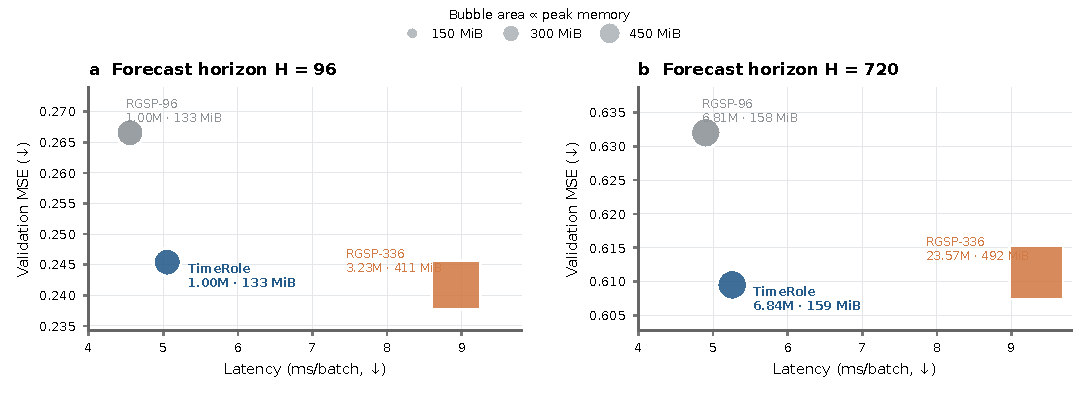
\includegraphics[width=\textwidth]{figures/Fig5_Efficiency_Tradeoff_v1.pdf}
\caption{Accuracy--efficiency trade-off of TimeRole on ETTm1 and ETTm2. \textbf{a,b} correspond to 96- and 720-step forecasting, respectively. The horizontal axis, vertical axis, and bubble area represent batch inference latency, validation MSE, and peak memory. Each point is the two-dataset average for random seed 2021; all methods use the same hardware, batch size, and checkpoint-evaluation procedure.}
\label{fig:efficiency-tradeoff}
\end{figure*}

Relative to RGSP-96, TimeRole increased the parameter count by approximately 0.5\%, batch inference latency by approximately 9.1\%, and peak memory by less than 0.5\%, while reducing the macro-average MSE over the four tasks by 5.215\%. Thus, DHC introduced distant history into the recent forecasting process with limited additional resource cost.

Compared with RGSP-336, TimeRole reduced the parameter count, inference latency, and peak memory by averages of 69.968\%, 43.503\%, and 67.735\%, respectively, while its four-task macro-average MSE was 2.046\% higher. RGSP-336 achieved a slightly lower average validation MSE for 96-step forecasting, whereas TimeRole performed better for 720-step forecasting. Compressing the distant history therefore avoided most of the resource growth incurred by directly extending the recent backbone and yielded a more balanced accuracy--efficiency profile.

\subsection{Discussion}

The primary function of TimeRole is not simply to increase the amount of visible history, but to separate historical coverage from the range processed by the high-resolution forecasting backbone. The controlled comparison with a shared recent backbone showed that DHC consistently improved the base forecast on the evaluated ETTm tasks. Frozen-parameter interventions further showed marked error increases when the distant history was mismatched with the current sample or when its observed trajectory was disrupted. Together, these findings support the intended division of roles: RGSP forms a base forecast from recent dynamics and cross-variable relationships, while DHC estimates an incremental correction from distant context aligned with the current state. The interventions demonstrate model dependence on distant content rather than causal identification of a particular temporal factor; they should therefore be interpreted as mechanism diagnostics, not causal evidence.

These results indicate that long-context forecasting depends not only on window length, but also on how limited modeling capacity is allocated across historical ranges. Previous work has shown that enlarging the input window does not necessarily improve forecasting accuracy \citep{Zhang2025MEW}. Consistent with this observation, longer distant coverage produced comparatively stable gains at long horizons, whereas enlarging the recent high-resolution window did not yield monotonic improvement. The small changes across distant pooling widths further indicate that distant history need not always enter the forecasting process at its original resolution. Using the recent window for fine-grained state modeling and compressing distant history into conditional memory preserves long-range context without forcing the recent backbone to scale with the total window. Historical range, representation resolution, and forecasting role should therefore be considered jointly.

The most stable gains arose from organizing the recent base forecast and distant conditional correction, rather than from a fixed advantage of every internal component across all tasks. Removing DHC consistently degraded system-level performance, while graph propagation, patch representation, and alternative correction parameterizations had dataset-dependent effects. The local advantages of several DHC variants also leave room to adapt the correction form. The TimeXer experiments further demonstrated that this history-routing strategy can be integrated with a different class of forecasting backbone and can outperform direct long input in most settings. Nevertheless, the ETTh2-720 result shows that compressed correction is not uniformly preferable across all data distributions and horizons. The resource results reveal a similar boundary: role differentiation can reduce parameter count and peak memory without necessarily reducing the realized inference latency of every backbone. The design is therefore most relevant when broad historical coverage is needed under model-capacity or memory constraints, while any speed advantage remains dependent on the backbone and operator implementation.

The present evidence has several limitations. The experiments use five regularly sampled datasets with no more than 21 variables, and the component and sensitivity analyses focus primarily on ETTm1, ETTm2, and Weather. The frozen-history interventions use a single checkpoint, and cross-backbone validation covers only TimeXer. TimeRole also employs a fixed recent--distant boundary, average-pooling width, and variable-wise correction coefficients shared across samples and forecast steps, preventing dynamic allocation of historical resolution according to the input state. The conclusions are therefore primarily applicable to regularly sampled multivariate long-term forecasting with a fixed history partition. Further evaluation is needed for higher-dimensional variables, missing or irregular observations, distribution shifts, and additional forecasting backbones. Dynamic boundaries driven by the recent state, data-dependent compression, and time-varying correction strengths are promising directions for extending history-role differentiation.

\section{Conclusion}

This paper presented TimeRole, a history-role-differentiated model for multivariate long-term time-series forecasting. TimeRole assigns distinct responsibilities according to the temporal distance of each observation from the forecast origin. RGSP preserves the original resolution of the recent window and produces a complete base forecast, whereas DHC compresses distant history and estimates an incremental correction conditioned on the recent state. This structure decouples the accessible historical range from the direct input length of the computationally intensive forecasting backbone.

Across five public datasets, four prediction horizons, and three random seeds, TimeRole achieved the lowest MSE in 11 tasks and the lowest MAE in 11 tasks, together with the best average rank for both metrics. Adding DHC reduced both MSE and MAE in all 24 dataset--horizon--seed comparisons that shared the same RGSP backbone, while frozen-checkpoint interventions showed that forecasting performance was closely associated with the distant content corresponding to the current sample. Historical-range sensitivity, transfer to TimeXer, and resource measurements further showed that compressed distant correction can expand historical coverage and, in most tasks, provide an accuracy--capacity trade-off distinct from both short recent input and direct long input. History-role differentiation therefore offers a resource-conscious approach to long-history modeling for regularly sampled multivariate long-term forecasting.
